\section{Columnar CP Prototypes}\label{sec:prototypes}

As a first (\texttt{v1}) prototype of this capability, a standalone columnar implementation of the ATLAS Egamma CP tool with zero-copy \texttt{nanobind} Python bindings was created to compute on-the-fly systematics variations for the dilepton system mass in $e^{+}e^{-}$ final states, $m_{ee}$.
Uproot was used to load PHYSLITE files of ATLAS $Z\to \ell\ell$ simulation into Awkward arrays, and the $e^{+}e^{-}$ event selections were applied with Coffea.
The columnar Egamma tool was initialized through the Pythonic interface, \texttt{atlascp.EgammaTools}, and then passed Awkward arrays of electrons to compute on-the-fly systematic variations of the electron reconstruction efficiency scale factors and energy correction resolution and scale.
The computations were additionally scaled out with \texttt{dask-awkward}~\cite{dask_awkward_2024} on the University of Chciago ATLAS Analysis Facility to minimize the compute wall time, with the gathered results visualized in~\Cref{fig:Zee_mc_systematics}.

This preliminary research was required as there was no ```zero action'' option to determine the viability of the proposed design \textit{a priori}.
The \texttt{v1} prototype established the foundations of what was possible with new tooling and that Pythonic interfaces to CP tools could be written without large amounts of work or deep knowledge of underlying CP tool design.
This showed a promising direction, but additional work was needed to achieve the necessary performance, integration, and support required for use.

A \texttt{v2} ``Columnar Athena'' prototype~\cite{columnar_athena} has been started to expand on the scope of the \texttt{v1} prototype.
This moves the development of the columnar tools and interfaces from individual standalone examples into a unified system under the ATLAS Athena framework~\cite{ATLAS_Athena} and migrates the ATLAS CP tools to a columnar backend with breaking the existing workflows using the EDM models.
It additionally adds infrastructure support for development of columnar analysis tools by adding \texttt{nanobind} to the ATLAS Externals tooling distributed as part of the ATLAS Athena Analysis Releases.
While currently under active development, the \texttt{v2} prototype will allow for full scale integration and performance tests of the columnar CP tools and interfaces.

\begin{figure}
    \centering
    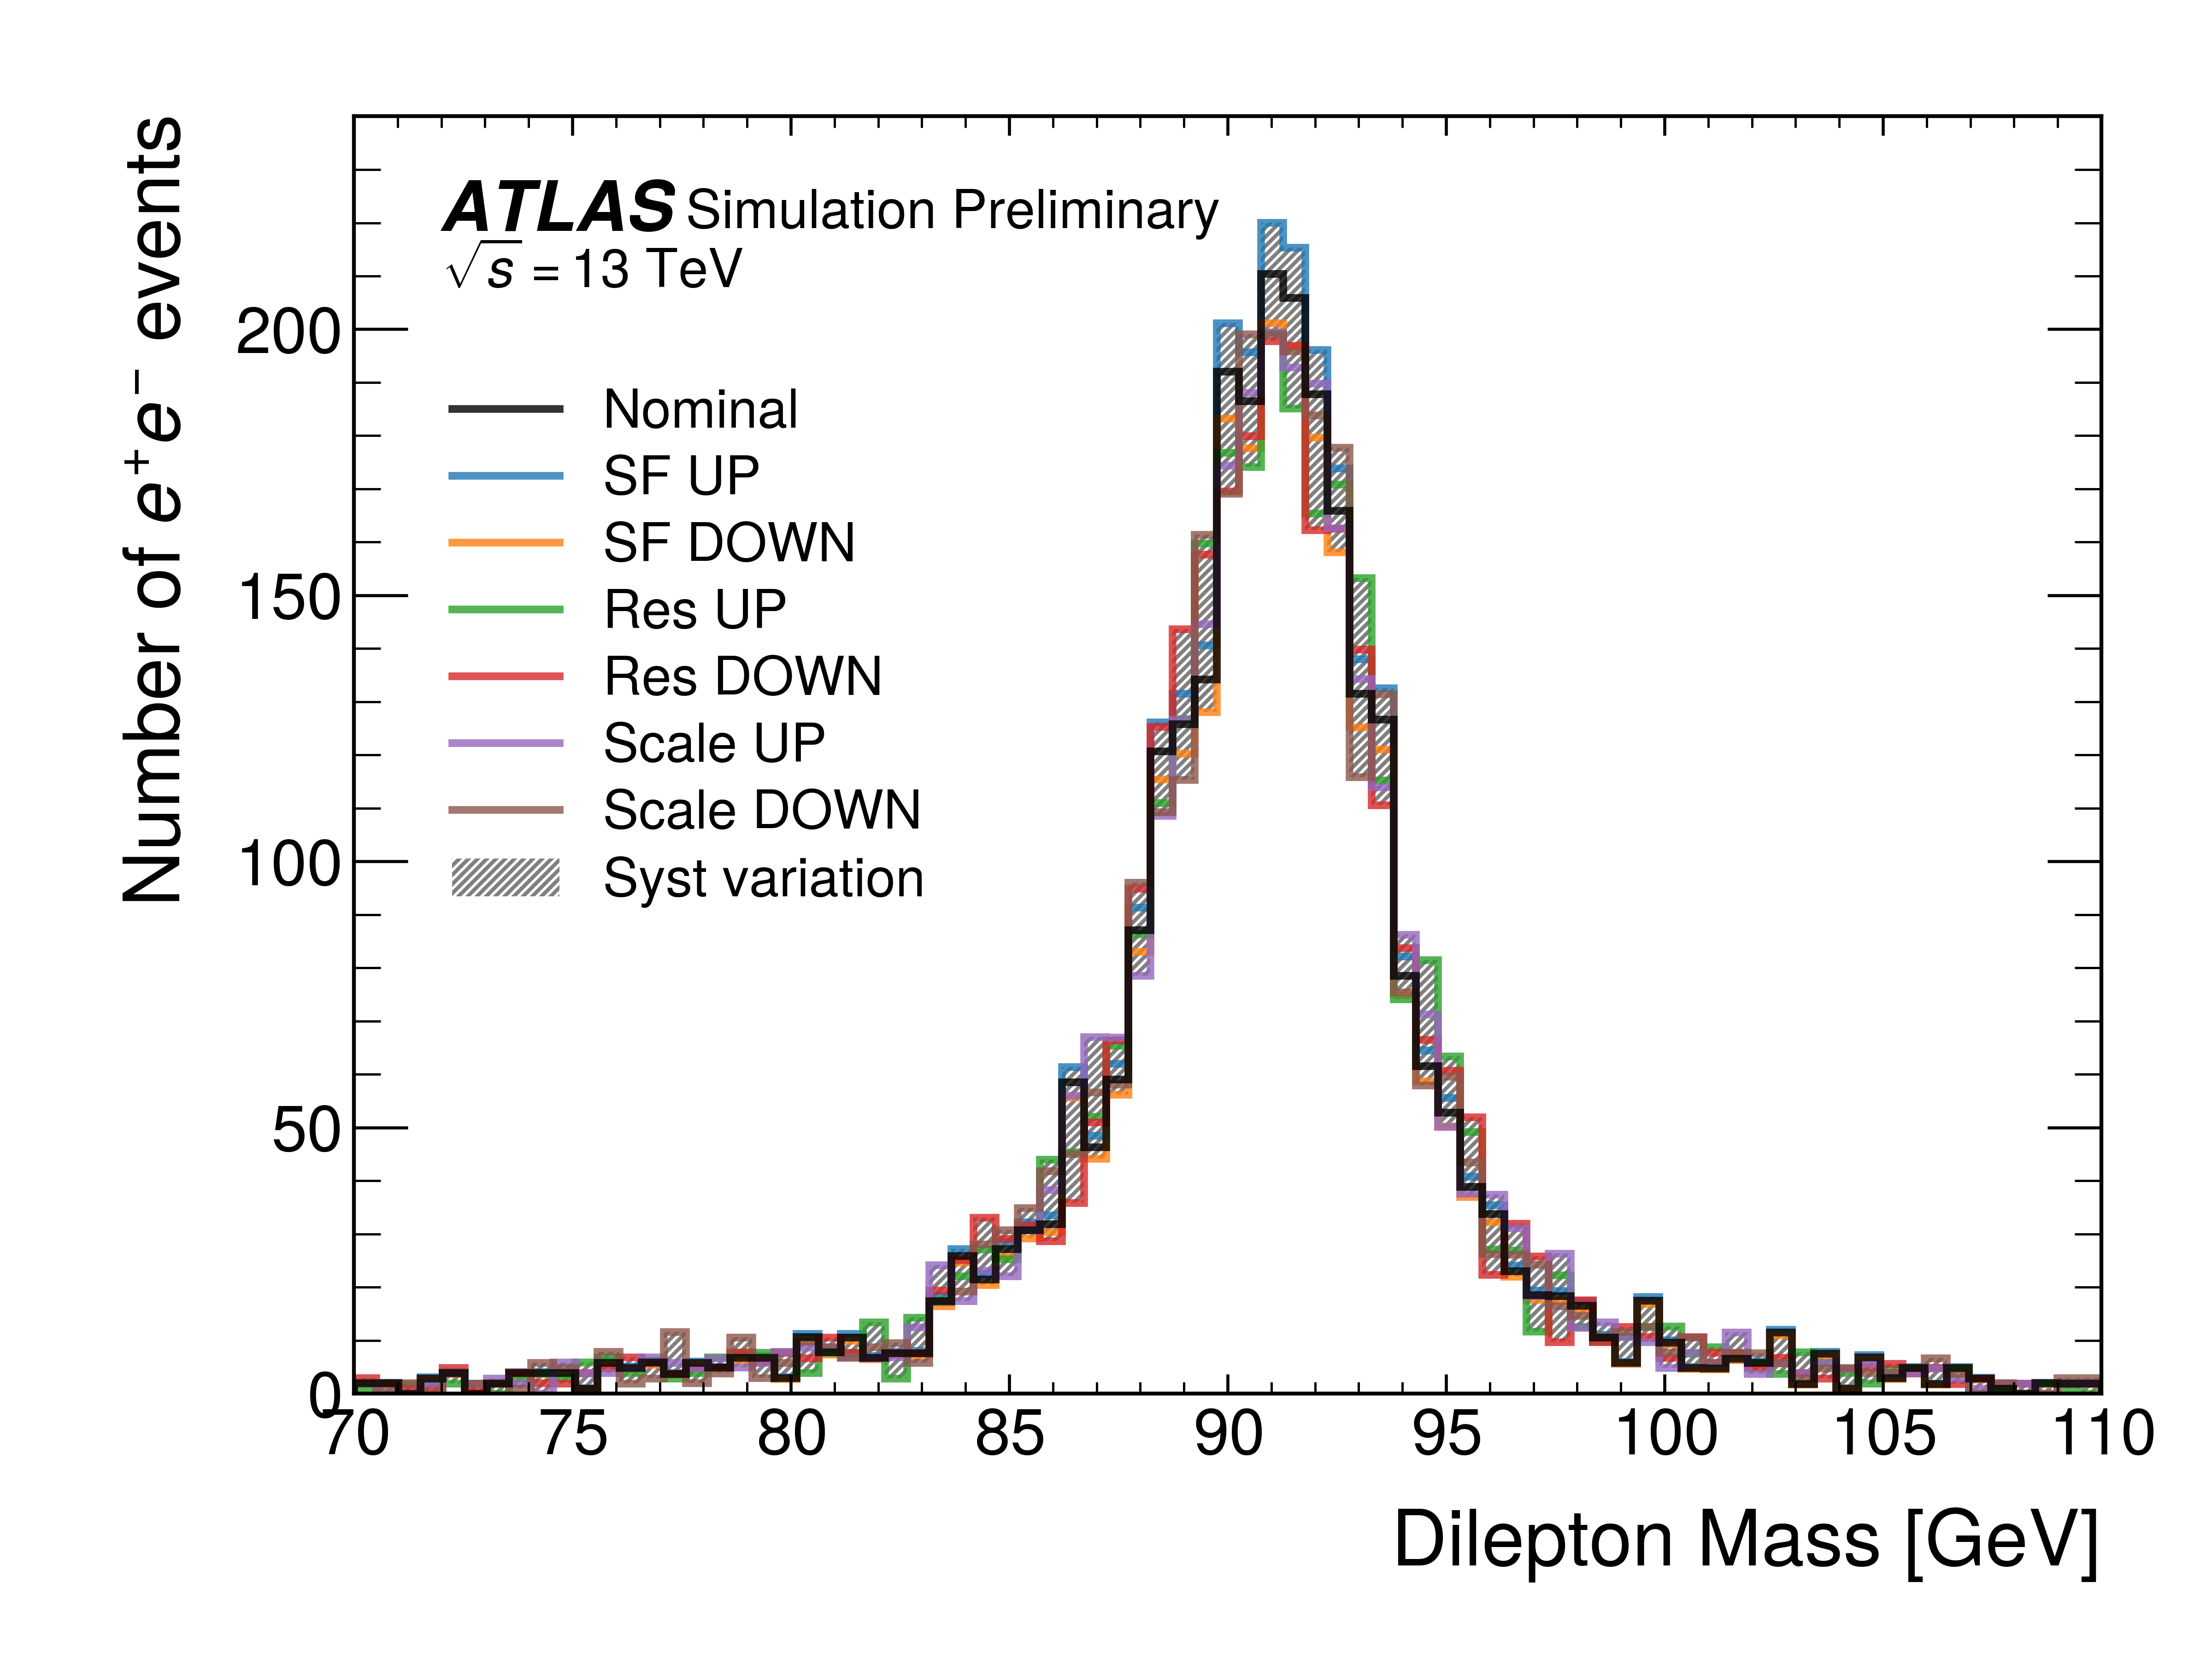
\includegraphics[width=0.7\textwidth]{Zee_mc_systematics.png}
    \caption{Histograms of the dilepton mass of selected $Z\to e^{+}e^{-}$ events in ATLAS simulation under on-the-fly systematic variations of the electron reconstruction efficiency scale factor (SF) --- the product of the reconstruction, identification, and isolation scale factors --- and energy correction resolution (Res) and scale (Scale)~\cite{Vigl:ACAT_2024}.}
    \label{fig:Zee_mc_systematics}
\end{figure}
